\documentclass[output=paper]{langscibook}
\author{Philothé Mwamba Kabasele\affiliation{University of Calgary; ISP/Gombe; University of Kwa-Zulu Natal}}
\title{Phonological adaptation of the Belgian French vowels in Kinshasa Lingala}
\abstract{This study provides a systematic analysis of vowel sound adaptations in KL with evidence from acoustic phonetics. The research is restricted to the phonological adaptations of vowel sounds from Belgian French (BF). It provides evidence from loan data on the existence of the contrastive features [±ATR] in KL phonological system. Questions raised include: does the phonological system of KL take precedence in the phonological adaptation process of the loanwords? Does similarity play a role in the adaptation of the loanwords? What happens when the foreign input does not offer any similarity with the phonological system of the recipient language (RL)? what happens when a feature/feature combination (FC) in a foreign input vowel either presents similarities with a feature/FC in the RL phonological system, or else does not present any similarities to any feature or FC in the phonological system of the RL? The data were extracted in a sentential context with a carrier sentence. Participants filled in the dots with the missing word that was suggested by the picture. The F1 and the F2 measurement values, in hertz (Hz) were taken at three different points of the vowel spectrogram. The script also generated the average measurement values which were considered as input for statistical analysis. The null hypothesis (Ho) predicts that BF [ɛ, œ, ø] would be adapted as [e] (Ho: [ɛ] = [e], [œ] = [e], and [ø] = [e]) in KL, while the alternative hypothesis (H1) predicts that the BF vowels [ɛ, œ, ø] would not be adapted as [e] (H1: [ɛ] ≠ [e], [œ] ≠ [e], and [ø] ≠ [e]) in KL. The Ho predicts that [ɔ] will be adapted as [o] (Ho: [ɔ] = [o]). Due to correlated nature of the data, Generalized Estimating Equation (GEE) was used to determine the degree of significant differences between two/more targeted variables. The findings have shown that KL speakers still discriminate between [ɛ] and [e], and [ɔ] and [o], which implies the existence of the underlying contrast between the features [+ATR] and [−ATR].}
\ChapterDOI{10.5281/zenodo.6906649}

\begin{document}
\maketitle

\section{Introduction}
The phonological adaptation of illicit foreign vowel sounds into Kinshasa Lingala (KL) linguistic system has received very little scholarly attention \citep{bambi1998preservation,mudimbe1977procedes}. There has been no systematic analysis of vowel sound adaptations in KL with evidence from acoustic phonetics, nor any explanation of these adaptations in terms of phonetics and its interface with phonology. Such analysis and explanation are the focus of the present study. The current study is restricted to the phonological adaptations of vowel sounds from Belgian French (BF), as this general dialect of French was the primary source of loanwords in Lingala. The main goal of this study is to provide evidence from loan data on the existence of the contrastive features [±ATR] in the phonological system of KL. The findings of this study serve as a diagnostic test.

This research is important because the findings of loanword adaptation allow linguists to understand the kind of cognitive transformation that a phonological system imposes to any linguistic input at the phonological level. It should be noted that an analysis which considers only native data may fail to account for the changes and fail to effectively capture the phonological system of the TL. An investigation of a phonological system with data from loanword adaptation is relevant in that the output of loanword adaptation reflects all facets of the phonological structure of a target language at the segmental, phonotactic, suprasegmental, and morpho-phonological level of the borrowing language \citep[1]{kang2011loanword}. Channeling \citet{berko1958child}, \citet[1]{kang2011loanword} suggests that “loanword phonology be considered as a real-life Wug test which can allow linguists to probe into the grammatical knowledge of speakers in ways that native data alone cannot”. Kang shows the real importance of a study in loanword adaptation and what could be its contribution in understanding the fine grain phonological system of a TL. Loanword adaptation can be used as a diagnostic test of the phonological preferences and constraints of a TL.

\begin{sloppypar}
Both integrated loanwords and on-line adaptations \citep{shinohara1997analyse} will be considered. On-line adaptations are loans which are borrowed “here and now” \citep[66]{calabrese2009loan} whereas integrated loanwords refer to those adopted forms which have been made part of the recipient language’s lexicon and whose source form appears to have been lost due to the phonological adaptation. The broad aim of this study is to identify various phonological strategies that Lingala speakers use when adopting and adapting BF vowels into their linguistic system. The study further aims to provide the phonetic-phonological motivation which justifies the choice of strategies during the loanword adaptation process and the different phonological constraints that regulate the adaptation process of vowels.
\end{sloppypar}

Previous research on loanwords \citep{mudimbe1977procedes,bambi1998preservation} relied strictly on phonological conditions in Lingala to explain the adaptation of French words in Lingala. This exclusive focus on Lingala phonology is understandable, but the leading experts in loanword phonology, LaCharité and Paradis, warn that the source language phonology plays an important and preponderant role in the process of adaptation (see, e.g., \citet{lacharite2005category}). They claim, as \citet[1]{kang2014french} put it, that “the adapters are competent bilinguals with native-like knowledge of the input language phonology and the phonological structure of the source language (SL) serves as input to the adaptation process, rather than the surface phonetic forms of the source language”. LaCharité and Paradis’s viewpoint is informed by multiple large-scale studies of loanword adaptation situations.

To make sense of vocalic adaptations in this study, among others, I will argue that three stages are involved in the adaptation process of an illicit input in the recipient language: the perceptual stage, the adaptation proper stage, and the implementation stage. The first and last stages are predominantly phonetically based. That is, phonetic factors play an important role in the adaptation process during these two stages. Yet the present study does not support the strictly phonetic approach to loanword adaptation which is advocated by \citet{peperkamp2003reinterpreting}, \citet{vendelin2004evidence}, and \citet{peperkamp2004psycholinguistic}, among others. This is because the adaptation proper stage is conceived as purely phonological. This is the stage in which the phonological constraints and preferences of the recipient language ‘paint’ their linguistic identity on the loanword to make it an accepted part of its linguistic system. I will suggest that loanword adaptation proper is a purely abstract process which leaves the speakers of a language with little choice. First, featural combinations which are similar between the SL input and the TL representation are generally preserved; this type of foreign input requires less cognitive effort since the SL features meet the phonological preferences of the TL.

Second, featural combinations which are dissimilar between the SL input and the TL representation are generally transformed and therefore sacrificed. This type of foreign input requires much cognitive effort since the SL features do not meet the phonological preferences of the TL. They may violate a number of the phonological constraints of the recipient language. Therefore, some repairs are imperative in order for the recipient language system to license the new linguistic form in the phonological system.

A third scenario concerns featural combinations that appear dissimilar between the SL input and the TL representation which may presage past and future preferences in the TL, as when certain phonological structures are admitted which have either been deactivated in the synchronic system of the language or have not yet previously been observed in the synchronic system. In this case the adapted linguistic form seems to reveal the reflexes of the diachronic system or seems to be ahead of its time in terms of the future linguistic preferences of the system and reveals the more abstract preferences of the language.

The next section provides some theoretical background on loanword adaptation. The following section briefly describes the research questions; section 4 is the study proper; section 5 the discussion and findings; and section 6 concludes the paper.

\section{Background}
\subsection{Considerations}
Phonological adaptation is a process that affects a loanword in order to make it conform with the linguistic ‘identity’ of the recipient language. Loanword (in the process of phonological adaptation) is defined as a word that has been borrowed from a linguistic system that is identified as the source language (SL) and is then integrated into a recipient linguistic system that is called the target language (TL). During the process of its integration, the borrowed word may or may not undergo a phonological adaptation which is mainly dictated by the phonological system of the TL that forces the loanword to abide by the phonological preferences and constraints of the recipient language.

A loanword is completely integrated in the borrowing language system when its illicit features become phonologically nativized in the TL in a way that its foreign pronunciation becomes unrecognizable. \citet[144]{thomason2001language} claims that some loanword adaptations  occur through the process of ‘negotiation’ which is identified by the phenomenon of correspondence rules or borrowing routines. Thomason argues that “correspondence rules are (mostly) phonological generalizations drawn, consciously or unconsciously by bilinguals, though full fluency in both languages is not required” (p. 144). He presents its generalization in the form “‘Your language has x where my language has y’ and the rules are generally applied to nativize the phonology of loanwords” (p. 144). \citet[139]{kenstowicz2006salience}, by contrast, claims that “[t]he adaptation of a loanword involves the resolution of often conflicting demands to preserve as much information from the source word as possible while still satisfying the constrains that make the lexical item sound like a word of the recipient language”. This way of looking at phonological adaptation may be too simplistic. The phonological adaptation process additionally involves complex abstract linguistic mechanisms that transform an illicit foreign input to abide by the linguistic preferences of the borrowing language. The phonological system of the recipient language – being a component of an autonomous linguistic system – is not obviously concerned about preserving the information from the source language. It may, but need not, preserve the linguistic features which abide by its phonological preferences in order to license its integration into the recipient linguistic system.

The adaptation that a loanword undergoes is a phonological transformation that results at the behest of the phonological system of the host language. The loanword has to abide by the phonological constraints and preferences of the TL. As \citet{kang2011loanword} puts it, “[s]uch adaptation affects all facets of phonological structure, reflecting the segmental, phonotactic, suprasegmental and morpho-phonological restrictions of the borrowing language” (p. 1). The output of the phonological adaptation process reflects “aspects of native speakers' linguistic knowledge” \citep[1]{kang2011loanword}. Loanword adaptation, therefore, allows linguists to understand the kind of cognitive transformation that a phonological system imposes to any linguistic input at the phonological level. Loanword adaptation can be used as a diagnostic test of the phonological preferences and constraints of the TL. It even reveals likely preferences that are not yet observed in the phonological system of the TL.

\subsection{Theories on loanword adaptation}
Though some ad hoc factors were identified in the literature on loanword adaptation, including orthography, morphology, and semantics (e.g. \citealt{vendelin2004evidence, Adler2006, DavisCho2006, Miao2006, Smith2006a, Smith2006b}), three broad approaches to phonological adaptations are pursued in the literature \citep{lin2009loanword}: the phonology approach, the perception approach, and the perception-phonology approach. This study adopts the perception-phonology approach.

\subsection{The perception-phonology approach}
A joint approach is proposed by \citet{Silverman1992}, \citet{Yip1993, Yip2004}, and \citet{Rose1999a, Rose1999b} who give credit to both the phonology and the perception approach by integrating the relevant features of the perceptual and the phonological components of the grammar. The perception-phonology approach claims that the input is shaped by the perceptual skills of the borrower, which determine how s/he decodes the acoustic signals of the source language. The adaptation process is dictated by the phonological system of the recipient language (e.g. \citealt{Silverman1992, Yip1993, Yip2002, Yip2006, Steriade2001, Kang2003, Kenstowicz2003, KenstowiczSuchato2006, Miao2006}).

While the perception-phonology approach claims that “the input to the adaptation process is based on how the borrowers perceive the acoustic signals of the source language” \citep[2]{lin2009loanword}, it does not identify the linguistic system that governs the perception of the foreign input. In other words, the approach does not predetermine whether the perception of a borrower is determined by the phonetic or phonological component of the language. Nor does it tell us whether the perceptual skills are part of the source language phonological system or whether it is the result of the recipient language phonological system. These questions are worth to clarify in order to shed light on the adaptation process of loanwords.

If we admit that adaptation is perceptual, we should equally admit that it is the phonological preferences (system) of the TL which interpret the foreign input in the way we perceive it. The phonological adaptation certainly starts at the perceptual level, but in turn it is dictated by the phonological preferences of the TL. For instance, if a foreign input is the aspirated stop [ph] and aspiration is not a preferred feature in the phonology of the TL (that is, it is not a component of the underlying representation of the language), native speakers of that TL may not perceive the aspiration because their grammar is unable to decode and interpret it as such. This is what \citet[6]{boersma2009loanword} argue: “perception is largely bound by native output constraints, so that a structure that violates native constraints cannot be perceived faithfully”.
Perceptual similarity is one of the most important cues in the process of loanword adaptation. It links the features of the foreign input to the features in the phonological system of the recipient language. \citet[6]{kang2011loanword} argues that “foreign input is faithfully perceived yet can nevertheless be adapted to adhere to native phonotactic constraints”.

This entails that the foreign input comes with its fully specified phonetic features which are adapted – or not – during the adaptation process. The input features that are similar to the phonological features in the recipient language are more likely to be adopted and preserved in the adaptation process than the input features which offer no similar matches in the recipient language.

\section{Research questions}
This study focuses on the phonological strategies used to adapt BF vowels in loanwords in Lingala, as spoken in the Congolese capital city of Kinshasa. Questions raised include: does the phonological system of KL take precedence (dictate its linguistic preferences) in the phonological adaptation process of the loanwords? Does similarity play a role in the adaptation of the loanwords? What happens when the foreign input does not offer any similarity with the phonological system of the recipient language? Of special interest is what happens when a feature or feature combination in a foreign input vowel either presents similarities with a feature or feature combination in the recipient language phonological system, or else does not present any similarities to any feature or feature combination in the phonological system of the recipient language?

The present study focuses on the BF vowels shown in \REF{ex:kabasele:1a}. All non-low vowels of KL are presented in \REF{ex:kabasele:1b}. Note that BF combines [+front] and [+round] in /y, ø, œ/, whereas this featural combination is disallowed in KL. Note, too, that the [−ATR] mid vowels /ɛ, ɔ/ are in parentheses in \REF{ex:kabasele:1b} because it is widely claimed that these vowels have fully merged with /e, o/ in KL (e.g., \citealt[20]{motingea2006}, \citealt[303]{bokamba2012polylectal},  \citealt[965]{campbell2013compendium}). If this is correct, the feature [±ATR] is not at all contrastive in KL phonology, whereas it is in BF.

\begin{exe}
\ex \label{ex:kabasele:1}
\begin{xlist}

\ex Selected vowels of Belgian French\label{ex:kabasele:1a}\\
\begin{tabular}{ccccc}
     &  & \multicolumn{2}{c}{[+\textsc{front}]} & [−\textsc{front}]\\
     &  & [−\textsc{round}] & [+\textsc{round}] & [+\textsc{round}] \\
 \ [+high] & [+\textsc{atr}] & /i/ & /y/ & /u/ \\[6pt]
  \multirow{2}{*}{[−high]} & [+\textsc{atr}] & /e/ & /ø/ & /o/ \\
  & [−\textsc{atr}] & /ɛ/ & /œ/ &  /ɔ/ \\[12pt]
\end{tabular}

\ex Non-low vowels of Kinshasa Lingala\label{ex:kabasele:1b}\\
\begin{tabular}{cccc}
  &    &  [+\textsc{front}] & [−\textsc{front}] \\
  &  & [−\textsc{round}] & [+\textsc{round}]\\
 \ [+high] & [+\textsc{atr}]    & /i/ & /u/ \\[6pt]
 \multirow{2}{*}{[−high]} & [+\textsc{atr}] & /e/ & /o/ \\
  & [−\textsc{atr}] & /ɛ/ & /ɔ/ \\
\end{tabular}

\end{xlist}
\end{exe}

\section{The study proper}
\subsection{Rationale}
The data were extracted in a sentential context with a carrier sentence which was structured as \textit{Nalobi……sikoyo} ‘I say…now’. Participants had to fill in the dots with the missing word that was suggested by the picture. The measurement values of these data were extracted at three different points such as at the beginning, middle and end of the formant and the automatically generated average values of each token were then computed by Praat. It is these average values which were considered for statistical analysis.

\subsection{Participants}
Eighteen subjects were recruited to elicit the data of this experiment. They all were native speakers of KL who were born and raised in Kinshasa. None of them has ever left Kinshasa. All of them could speak some French. Their ages varied between 18 and 57 years old. None of them had any problem in articulation. They all were healthy at the time they performed the tasks of this study. \tabref{tab:subjects} presents the demographic of the subjects of this experiment.

\begin{table}
    \resizebox{\textwidth}{!}{\begin{tabular}{l cccccccc}
    \lsptoprule
          & \multicolumn{4}{c}{Younger than 37} & \multicolumn{4}{c}{Older than 37} \\
      \midrule
       Age range & \multicolumn{2}{c}{18–27}  & \multicolumn{2}{c}{28–37} &  \multicolumn{2}{c}{38–47} & \multicolumn{2}{c}{48–57}\\
       Gender & Male & Female & Male & Female & Male & Female & Male & Female \\
       Total & 3 & 	2 & 	2 & 	2	& 	1 & 	2 & 	3 & 	3 \\
       Subtotal & \multicolumn{2}{c}{5} & \multicolumn{2}{c}{4} & \multicolumn{2}{c}{3} & \multicolumn{2}{c}{6} \\
       Total & \multicolumn{4}{c}{9} & \multicolumn{4}{c}{9} \\
       Grand total & \multicolumn{8}{c}{18} \\
       \lspbottomrule
    \end{tabular}}
    \caption{The demographics of the subjects\label{tab:subjects}}
\end{table}

\subsection{Research hypothesis}
Six pairs of vowels were compared in this study. The predictions of all the experiments were formulated on the basis of my assumptions which support the claim that when a segment does not exist in the linguistic system of the TL, the illicit segment is adapted to the closest form that exists in the linguistic system of the recipient language (see \citealt{kang2011loanword} for discussion).

The predictions of this study are, for instance, that Belgian French mid vowels /ɛ/, /œ/, /ø/ will be adapted as /e/ with some initial input matching feature(s) preserved in the recipient language if and only if the said feature(s) also exist(s) in its phonological system; or with those features sacrificed if they are not preferred in the phonological system of the recipient language. That is, BF /ɛ/ would be adapted as /e/ in KL if and only if the phonological system of KL disprefers the phonological features of the input /ɛ/.
On the assumption in the literature that /ɛ/ is merged into /e/ in KL \citep{motingea2006,bokamba2012polylectal,campbell2013compendium} , the closest BF medial vowel form in KL would be [e], since [ɛ]
is assumed to no longer exist in the system. Therefore, the null hypothesis predicts that BF [ɛ, œ, ø] would be adapted as [e] (H\textsubscript{o}: [ɛ] = [e], [œ] = [e], and [ø] = [e]) in KL, while the alternative hypothesis predicts that the Belgian French vowels [ɛ, œ, ø] would not be adapted as [e] (H1: [ɛ] ≠ [e], [œ] ≠ [e], and [ø] ≠ [e]) in KL.

Along the same lines, the null hypothesis predicts that [ɔ] will be adapted as [o] (H\textsubscript{o}: [ɔ] = [o]). That is, KL speakers will adapt [ɔ] = [o]) since the latter vowel is closer to the formerly mentioned illicit input [ɔ]. Whereas, the alternative hypothesis predicts that [ɔ] will not be adapted as [o] (H\textsubscript{1}: [ɔ] ≠ [o]).

I argue in this study that the adaptation process of a foreign input that is illicit in the TL is a gradient process which abides by a number of constraints that are hierarchically ranked in the phonological system of the recipient language, of which the phonetic-phonology feature matching and mapping that observe the phonological preferences of the TL tend to be universally ranked higher. According to this perspective, the process of phonological adaptation tends to preserve the highly ranked preferred foreign phonetic-phonology feature into the phonological system of the TL. The hypotheses of the 6 pair tests are presented in \tabref{tab:hypothesis}.


\begin{table}
    \begin{tabular}{ccccc}
    \lsptoprule
         &  &  & \multicolumn{2}{c}{Hypothesis} \\\cmidrule(lr){4-5}
       Exp.  & Pair & Formant & H\textsubscript{0} & H\textsubscript{1} \\
       \midrule
       \multirow{2}{*}{1} & \multirow{2}{*}{[ɛ] vs. [e]} & F1 &  F1 of [ɛ] = F1 of [e] &  F1 of [ɛ] ≠ F1 of [e] \\
       & & F2 &  F2 of [ɛ] = F2 of [e] & 	 F2 of [ɛ] ≠ F2 of [e]\\
       \midrule

       \multirow{2}{*}{2} & \multirow{2}{*}{[ø] vs. [e]} & F1 & 	 F1 of [ø] = F1 of [e] & 	 F1 of [ø] ≠ F1 of [e]\\
         & & F2	&  F2 of [ø] = F2 of [e] & 	 F2 of [ø] ≠ F2 of [e]\\
         \midrule

     \multirow{2}{*}{3} & \multirow{2}{*}{[œ] vs. [e]} & F1	&  F1 of [œ] = F1 of [e] & 	F1 of [œ] ≠ F1 of [e] \\
       & & F2 & 	 F2 of [œ] = F2 of [e] & 	 F2 of [œ] ≠ F2 of [e] \\
       \midrule

     \multirow{2}{*}{4} & \multirow{2}{*}{[ɛ] vs. [œ]} & F1	&  F1 of [ɛ] = F1 of [œ] & 	 F1 of [ɛ] ≠ F1 of [œ] \\
     & & F2 & 	F2 of [ɛ] = F2 of [œ] & 	 F2 of [ɛ] ≠ F2 of [œ] \\
     \midrule

     \multirow{2}{*}{5} & \multirow{2}{*}{[ɛ] vs. [ø]} & F1	&  F1 of [ɛ] = F1 of [ø] & 	 F1 of [ɛ] ≠ F1 of [ø] \\
     & & F2	&  F2 of [ɛ] = F2 of [ø]	& F2 of [ɛ] ≠ F2 of [ø] \\
     \midrule

     \multirow{2}{*}{6} & \multirow{2}{*}{[ɔ] vs. [o]} & F1	& F1 of [ɔ] = F1 of [o]	&  F1 of [ɔ] ≠ F1 of [o] \\
                                                    & & F2	& F2 of [ɔ] = F2 of [o]	&  F2 of [ɔ] ≠ F2 of [o] \\
     \lspbottomrule
    \end{tabular}
    \caption{Research hypothesis\label{tab:hypothesis}}
\end{table}

\subsection{Data analysis}
The Praat program\footnote{Computer program, version 6.0.14 11 retrieved February 2016 from \url{http://www.praat.org/}.} was used to measure the values of the F1 and F2 to determine the degree of the height and frontness\slash backness of the targeted vowels in the whole study. The measurement values, in hertz (Hz), of the F1 and the F2 were taken at three different points of the vowel spectrogram. The script also generated the average measurement values which were considered as input for statistical analysis.

Due to correlated nature of the data, Generalized Estimating Equation (GEE) was used to determine the degree of significant differences between two or more targeted variables. For instance, the F1 values of the adapted [ɛ] (i.e., KL vowel adapted from BF [ɛ]) were compared to the F1 values of adapted [e] (i.e., KL vowel adapted from BF [e]) to determine whether they were significantly different; the same procedures were used for the F2 values of the adapted [ɛ] and the adapted [e] to determine whether they were significantly different. The next section presents the results of different pair tests.

\subsection{Evidence that participants were in KL linguistic mode when producing the target vowels}\largerpage
How does a researcher make sure that bilingual or multilingual participants are in the target language linguistic mode when producing the target vowels in the study? Five types of evidence are presented here as robust evidence on the fact that the vowels that were produced by KL speakers in this study were effectively adapted vowels in KL, but not French vowels.

First, to make sure that the bilingual speakers were in KL linguistic mode \citep{grosjean2001bilingual}, but not in French linguistic mode, all the research was conducted in KL. That is, all the interactions and instructions were in KL. This technique was used by Grosjean in his study on mixed language processing, in which he strictly controlled for the language mode factor. He specifically told the participants that he was doing research on mixed language (code-switching, borrowing), he interacted with them in mixed language, and asked them to keep their two languages on at all times (pp. 412--413). Besides, subjects in the current study were specifically asked to produce those words in KL the way they always do it while speaking in Lingala. The fact of specifying the language – Kinshasa Lingala – in which they had to produce those words, puts them in KL linguistic mode.

\citet[2]{grosjean2001bilingual} defines language mode as “[t]he state of activation of the bilingual’s languages and language processing mechanisms at a given point in time”.  For example,  if you ask a French-English bilingual speaker to produce the word courage in French, s/he will read it as /kuˈraʒ/, but not as /ˈkɜrɪd͡ ʒ/ even if the subject speaks both French and English. Likewise, if you ask him/her to produce the same word in English, s/he will read it as /ˈkɜrɪd͡ ʒ/, but not /kuˈraʒ/. The specified language and the word that is produced abide by a particular phonological system. This phonological match entails that when a bilingual speaker is asked to produce a word in a specific language, s/he regulates her/his speech production according to the linguistic mode of that particular language.

\citet[410]{grosjean2003processing} says, “At the monolingual end of the continuum, bilinguals adopt the language of the monolingual interlocutor(s) and deactivate their other language (s) as best as possible”. The mere fact of specifying the language in the instruction helps the bilingual subject to switch into the appropriate language mode that is associated with the specific language. Grosjean further states “when the bilingual is in a monolingual mode, one can assume that the other language is not activated.” \citet[412]{Green1986} even proposed that the other language is “inhibited”. Third, even if those words look French in their orthography, they have been fully integrated in KL and do not have an alternative in the language. For instance, if you ask a KL speaker to give you the Lingala word for `a window' or `a door', s/he will most certainly say \textit{fenetre} ‘window’ or \textit{porte} ‘door’ respectively. These words have been fully integrated in the KL lexical system that the original words are just lost and unknown to speakers. Fourth, evidence that my subjects were in KL linguistic mode further came from the data of this study (pilot study) in which 5 subjects were asked to produce those words first in Lingala, and then in French. In the first mini experiment, subjects were asked to produce 11 words in Lingala. In the second experiment, they were asked to produce those same words in French. The results are produced in \tabref{tab:pilot}.

\begin{table}
    \begin{tabular}{*4{l}}
    \lsptoprule
     & \multicolumn{3}{c}{Speakers' production}\\\cmidrule(lr){2-4}
     & \multicolumn{1}{c}{BF} & \multicolumn{2}{c}{{KL}} \\\cmidrule(lr){2-2}\cmidrule(lr){3-4}
    {Words} & {In French} & {In French} & {In Lingala}  \\\midrule
    caleçon  & [kalsɔ̃]& [kalsɔ̃] (3),  & [kal\textit{e}sɔ̃] (5) \\
    `underwear' & & [kal\textit{e}sɔ̃] (2) & \\
    \tablevspace

    bracelet & [braslɛ] & [brasle] (1)  & [bras\textit{e}le] (5) \\
    `bracelet' & & [bras\textit{e}le] (4) & \\
    \tablevspace

    cambiste & [kɑ̃bist] & [kɑ̃bist] (2) & [ka\textsuperscript{m}bist\textit{e}] (5)\\
    `trader'  & & [kãbist\textit{e}] (1) , & \\
    & & [ka\textsuperscript{m}bist\textit{e}] (2) & \\
    \tablevspace

    chapelet & [ʃaplɛ] & [ʃaple] (2) & [ʃap\textit{i}le] (1) \\
    `rosary' &  & [ʃap\textit{e}le] (3) & [ʃap\textit{e}le] (4) \\
    \tablevspace

    chomeur & [ʃomœr] & [ʃomer] (2) & [ʃomer\textit{e}] (5) \\
   `jobless person' & & [ʃomer\textit{e}] (3) & \\
    \tablevspace

    ceinture & [sɛ̃tyr] & [sɛ̃tir] (3) & [sɛ̃tir\textit{e}] (5) \\
    `belt' & & [sɛ̃tir\textit{e}] (2) & \\
    \tablevspace

    centenaire & [sɑ̃tnɛr] & [sɑ̃tner] (1) & [sɑ̃t\textit{e}ner\textit{e}] (5) \\
    `centenary' & & [sɑ̃t\textit{e}ner] (2) & \\
    & & [sɑ̃t\textit{e}ner\textit{e}] (2) & \\
    \tablevspace

    chaussette & [ʃosɛt] & [ʃoset] (2) & [ʃoset\textit{e}] (4) \\
    `socks' & & [ʃoset\textit{e}] (3) & [ʃoset\textit{i}] (1) \\
    \tablevspace

    brosse & [brɔs] & [brɔs] (1) & [bros\textit{e}] (5) \\
    `brush' &  & [brɔs\textit{e}] (4) & \\
    \tablevspace

    rechaud & [reʃo] & [reʃo] (5) & [reʃo] (5) \\
    `cooker' & & & \\
    \tablevspace

    avion & [avjɔ̃] &  [avjɔ̃] (3) & [av\textit{i}jɔ̃] (5) \\
    `airplane' & & [av\textit{i}jɔ̃] (2) & \\
    \lspbottomrule
    \end{tabular}
    \caption{Word transcription as produced by KL speakers in the pilot study}
    \label{tab:pilot}
\end{table}

Note that italic emphasis refers to the epenthetic vowels as produced by KL speakers. The results in \tabref{tab:pilot} show that when KL speakers are in KL linguistic mode, they usually insert an epenthetic vowel after a coda to break the illicit sequence of CC within a word, resulting in the re- syllabification of the coda into an onset. The same is observed with the final coda which is re- syllabified as an onset. In some cases, there is shift of the stress from the left to the right-hand side, to the adjacent juxtaposed syllable as in [ˈkalsɔ̃] \to [kaˈlesɔ̃] and [ˈavjɔ̃]
\to [aˈvijɔ̃]. These results once more confirm that when the language to use by the participants is specified in the instruction and the interaction in a monolingual mode, the bilingual speakers switch to the linguistic mode of the target language and fully activate the base/matrix language, which in this case is KL. The differences in their production between BF and KL were rather intriguing, as shown in \tabref{tab:pilot}. Fourth, I also used my intuition as a native speaker of KL to determine whether subjects were in KL linguistic mode or not. For instance, whenever a subject would insert an epenthetic vowel in a word to break the sequence of coda-onset, that was an intuitive indication that the subject was in KL linguistic mode, since in most cases KL does not allow a coda in a syllable. These linguistic realities are robust evidence that my subjects produced the target vowels in this study in KL.

\subsection{The results}
The results of the Generalized Estimating Equation (GEE) comparing the F1 and F2 values of the pairs of the adapted target vowels are presented in \tabref{tab:table4}.

\begin{table}
% % % \begin{sideways}
% % %     \centering
% % %     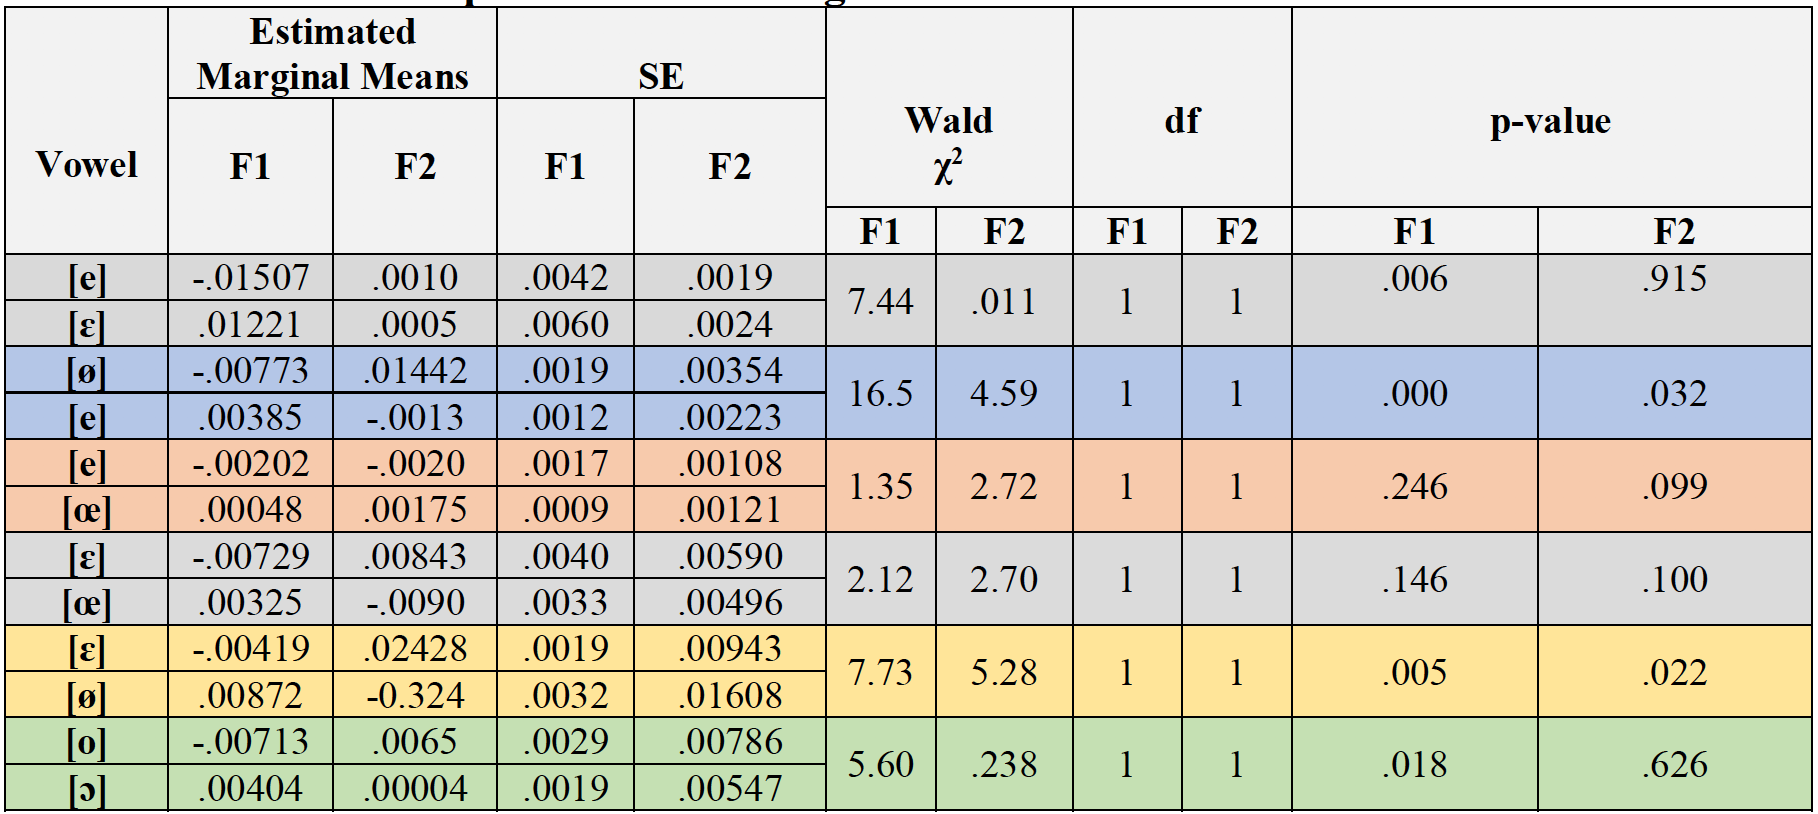
\includegraphics[scale=0.5]{figures/kabasele-table4.png}
% % % \end{sideways}
    \caption{The results for the comparisons of the target vowels\label{tab:table4}}
	\fittable{\begin{tabular}{l *2{S[table-format=-1.5]}  *2{S[table-format=1.4]} S[table-format=2.2] S[table-format=1.2] cc *2{S[table-format=1.3]}}
	\lsptoprule
	          & \multicolumn{2}{c}{EMM\footnote{Estimated marginal means}} & \multicolumn{2}{c}{SE} & \multicolumn{2}{c}{Wald $\chi^2$} & \multicolumn{2}{c}{df} & \multicolumn{2}{c}{$p$}\\\cmidrule(lr){2-3}\cmidrule(lr){4-5}\cmidrule(lr){6-7}\cmidrule(lr){8-9}\cmidrule(lr){10-11}
		           & {F1} & {F2} & {F1} & {F2} & {F1} & {F2} & {F1} & {F2} & {F1} & {F2}\\\midrule
		\relax [e] & -.01507 & .0010   & .0042  & .0019   &  7.44 & .011  &  1 & 1  & .006 & .915\\
		\relax [ɛ] &  .01221 &  .0005  & .0060  & .0024   &       &       &    &    &      &     \\\midrule
		\relax [ø] & -.00773 &  .01442 &  .0019 &  .00354 &  16.5 &  4.59 &  1 &  1 & .000 & .032\\
		\relax [e] & .00385  & -.0013  & .0012  & .00223  &       &       &    &    &      &     \\\midrule
		\relax [e] & -.00202 &  -.0020 &  .0017 &  .00108 &  1.35 &  2.72 &  1 &  1 & .246 & .099\\
		\relax [œ] & .00048  & .00175  & .0009  & .00121  &       &       &    &    &      &     \\\midrule
		\relax [ɛ] & -.00729 &  .00843 &  .0040 &  .00590 &  2.12 &  2.70 &  1 & 1  & .146 & .100\\
		\relax [œ] & .00325  & -.0090  & .0033  & .00496  &       &       &    &    &      &     \\\midrule
		\relax [ɛ] & -.00419 &  .02428 &  .0019 &  .00943 &  7.73 &  5.28 &  1 &  1 & .005 & .022\\
		\relax [ø] & .00872  & -0.324  & .0032  & .01608  &       &       &    &    &      &     \\\midrule
		\relax [o] & -.00713 &  .0065  & .0029  & .00786  & 5.60  & .238  & 1  & 1  & .018 & .626\\
		\relax [ɔ] & .00404  & .00004  & .0019  & .00547  &       &       &    &    &      &     \\
    \lspbottomrule
	\end{tabular}}
\end{table}

These results in \tabref{tab:table4} reflect the pairwise comparisons of estimated marginal means based on the original scale of dependent variables zF1 and zF2 for the pairs of target vowels. The results of the Wald chi-square that tested the simple effects of vowel within each level combination of the other factors shown which was based on the linearly independent pairwise comparisons among the estimated marginal means for F1 and F2 are presented in \tabref{tab:table4}.

It should be noted that only the results of the F1 accounts for the raising of the target vowel in the adaptation process, which entails that merger or neutralization of two segments is accounted for by only the results of the F1. The F2 served to determine the degree of either frontness or backness of the vowel. It also helped to account for the unrounding of any target vowel.

\section{Findings of BF vowel adaptation in KL}
The global findings of this experiment show that the adapted front and back mid-vowels /ɛ/ and /e/, and /ɔ/ and /o/ have been adapted as separate segments [ɛ] and [e], and /ɔ/ and /o/ respectively. These pairs of vowels have been adapted in different phonetic spaces. This is evidence of the existence of contrast between [+ATR] and [−ATR] in the phonological system of KL.

This adaptation process preserves the phonological features which are already licensed within a particular perimeter of the phonological/ phonetic space of KL. In clear, the [−round] which is licensed within the front perimeter of the phonological/ phonetic space of KL is preserved as well as the [+round] within the back phonetic space of KL.

The phonological adaptations of both [ɛ] and [e] as two distinct segments in KL provides an interesting evidence in favor of the existence of these segments as distinct phonological entities in the abstract representation of KL. If that were not the case, the contrast between these two segments would not have emerged. This findings on the non-merger of [ɛ] and [e] during their adaptation process in KL shows and challenges the claim in the existing literature that these two vowels are merged in KL.

In the back phonetic space of KL, the BF pair of vowels /ɔ/ and /o/ have been adapted as two different segments in the system. The survival of the phonological contrast between the  pair of vowels /ɔ/ and /o/ offers interesting evidence to build the story against the claim in the existing literature that /ɔ/ and /o/ are merged in KL.

However, /œ/ has been adapted as both [e] and [ɛ]. This implies that /œ/ has been adapted within the loop of the intersection point that has been created through the process of contrast reduction of [e] and [ɛ]. It is assumed from this phonological adaptation that [ɛ] and [e] overlap at a certain point of their phonetic space to an intersection surface that is not wide enough for both sound to merge. However, the intersection point of their overlap is the space within which [œ] is adapted. As a result, [œ] is adapted in their phonetic spaces scarifying its initial feature such as [+round]. Figure \ref{fig:1} illustrates the adaptation of [œ] into both [ɛ] and [e].


\begin{figure}
    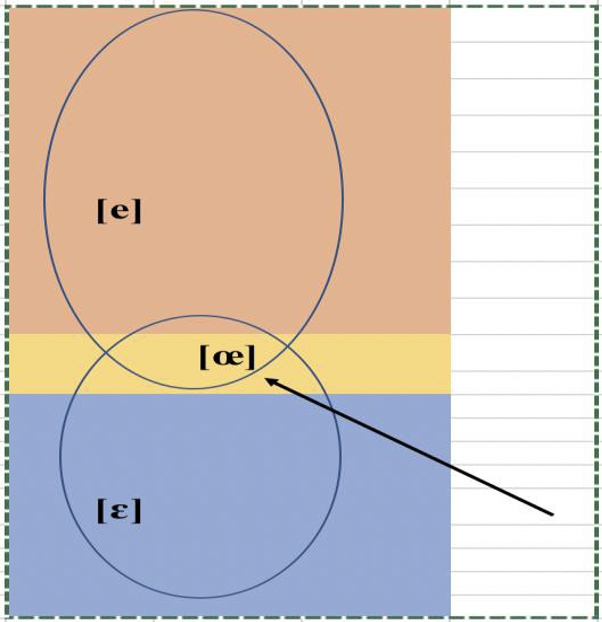
\includegraphics[width=.5\textwidth]{figures/kabasele-figure1.png}
    \caption{The adaptation of [œ] into both [ɛ] and [e]}
    \label{fig:1}
\end{figure}

Besides, /ø/ has been adapted in different phonetic spaces than [e] and [ɛ]. The non-merger of /ø/ with neither [ɛ] nor [e] entails that KL has adopted a new segment in its phonological/ phonetic system. This segment does not obey the phonological constrains of KL within the front parameter space of KL phonetic space. Such is the case of the combination of [+round] and [+front] with native data in KL.

It should be recalled that the adaptation process of [ø] into KL phonological/ phonetic space reveals some exceptional cases which do not obey the phonological patterns of the adaptation process of BF vowels in KL. In all the cases, the adaptation process of a BF vowel in KL prohibits the combination of [+round] with [+front] yet this combination is possible only when [ø] is adapted in KL. Second, in all the aforementioned cases, the combination of [+ATR] and [+round] in the front-parameter of KL phonetic space is constrains, yet with the adaptation of [ø] these constrains are violated. Could we consider [ø] as a transparent segment which does not obey any constrains during its phonological adaptation process in KL?

I posit that a transparent segment is the one which displays exceptional phonological behavior during its given phonological process resulting in a violation of the identified and attested constraints that regulate the phonological process of a target language. Such is therefore the case of the phonological adaptation of the BF [ø] in KL.

It should be also pointed out that the fine-grained phonetic traces of the BF are preserved somewhat and can still be traced back in the phonetic space of KL. These original fine-grained phonetic traces of the BF that are still identified in KL phonetic space are to be considered as the linguistic vestige (remnant) of this adaptation process. This linguistic vestige is the case of [+round] of [ø] which has been preserved during the adaptation process. The findings of this study are illustrated in \figref{fig:2}.

\begin{figure}
    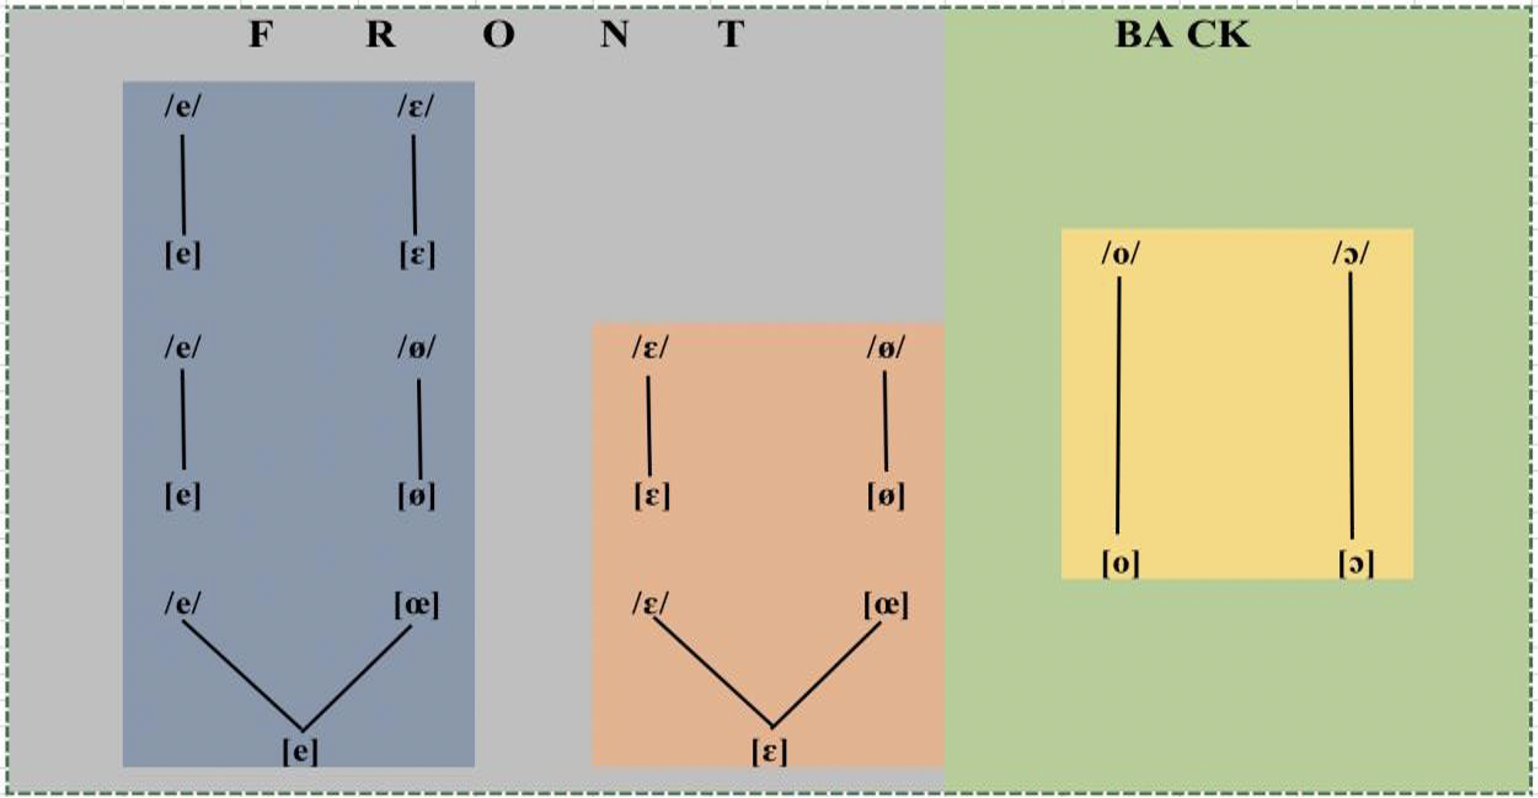
\includegraphics[width=\textwidth]{figures/kabasele-figure2.png}
    \caption{Global findings of BF vowel adaptation in KL in terms of segments}
    \label{fig:2}
\end{figure}

The findings in Figure \ref{fig:2} could be otherwise represented and discussed in terms of features. Unlike with the native data (automatically extracted data) which showed that KL does not accept [−ATR] in the back phonetic space of KL linguistic system, the findings of the adapted vowels show the opposite. In fact, these findings show both [+ATR] and [−ATR] are preferred in the system. However, the findings of the front phonetic space from native data disagree with the findings of the adapted vowels in KL. KL native data system attests the preference of both [+ATR] in front phonetic space of the system, while the Loan data system shows preference to both [+ATR] and [−ATR]. These realities are represented in Figures~\ref{fig:3} and~\ref{fig:4}.

\begin{figure}
    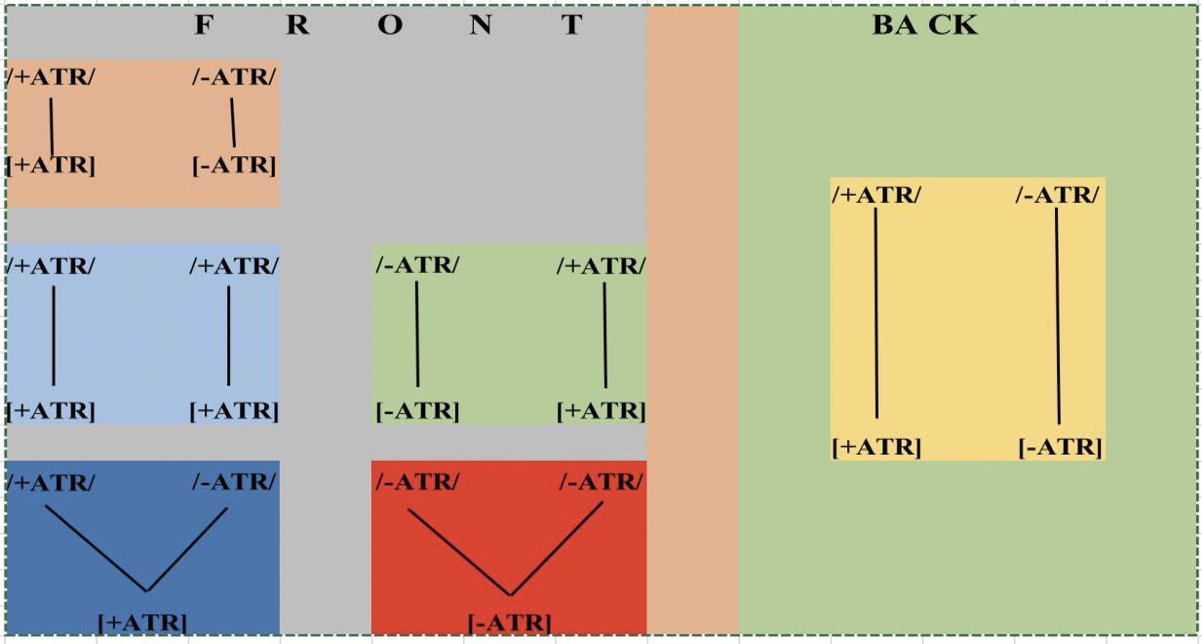
\includegraphics[width=\textwidth]{figures/kabasele-figure3.png}
    \caption{Findings of BF vowel adaptation in KL in terms of [+/−ATR] features}
    \label{fig:3}
\end{figure}

\begin{figure}
    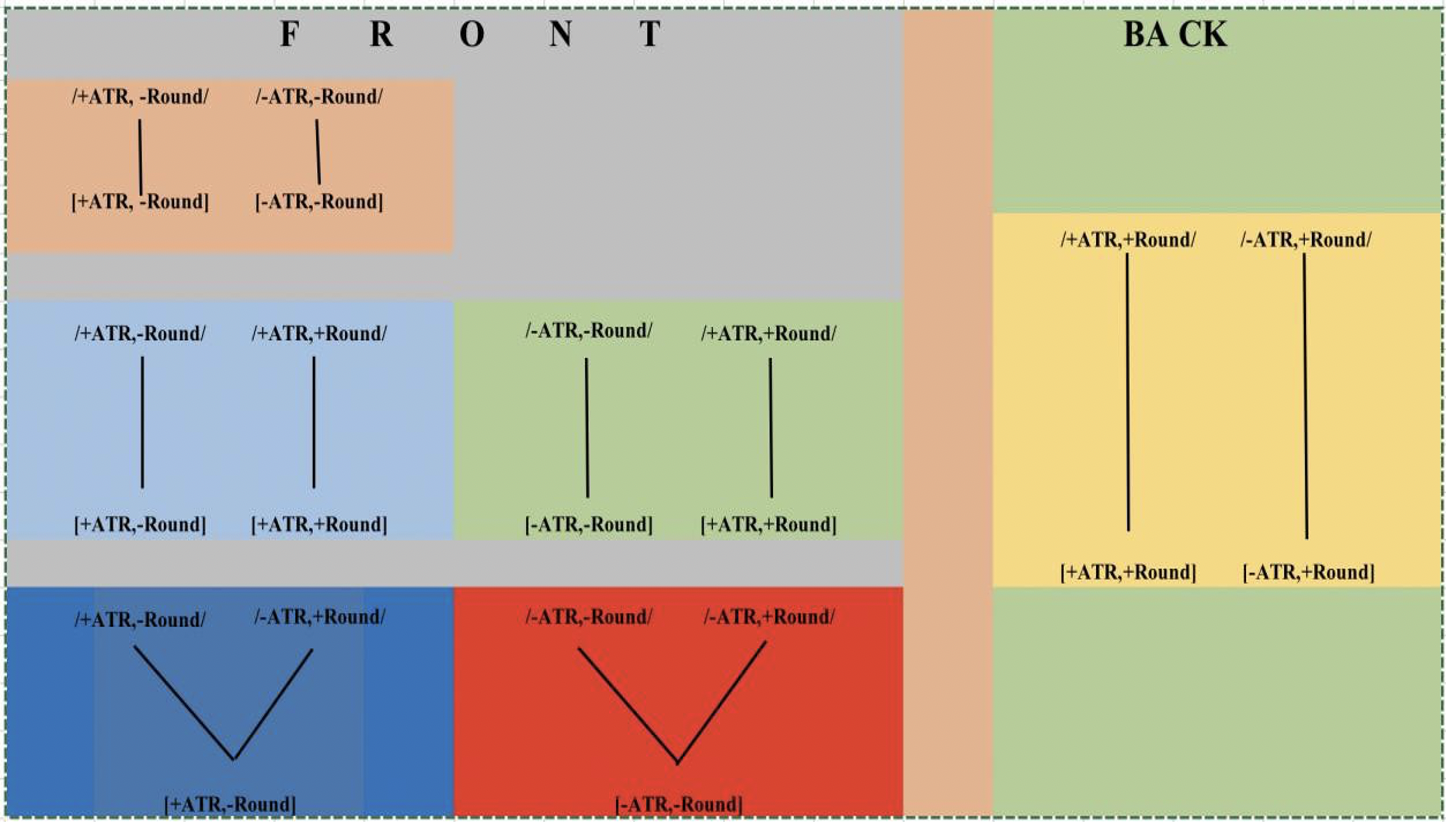
\includegraphics[width=\textwidth]{figures/kabasele-figure4.png}
    \caption{Findings of BF Vowel Adaptation in KL in Terms of [+/−ATR] and [+/−round] Features}
    \label{fig:4}
\end{figure}

\section{Conclusion}
The global findings of loanword adaptation in KL help to build a story in either support or rejection of a number of concerns that were raised in this study. They help to provide further evidence in rejection of the claim that KL speakers do not make any differences between the mid-vowels [ɛ] and [e], and [ɔ] and [o].

In fact, the findings of this study have shown that KL speakers still discriminate between the pairs of vowels [ɛ] and [e], and [ɔ] and [o], which implies the existence of the underlying contrast between the features [+ATR] and [−ATR]. Such evidence could be used as a recoverability diagnostic evidence to the process of non-merger of /o/ and /ɔ/ in KL native data as claimed in the existing literature. By showing through this study that the process of BF mid-vowel adaptation displays contrast, these findings help to further argue for the existence of the contrast even at the underlying representation of KL.

Referring back to the research questions that were raised earlier in this study, it is shown that the phonological system of KL primarily dictates its linguistic preferences in the phonological adaptation process of the loanwords in KL. The evidence comes from the fact that most of the adapted vowels from the BF obey the phonological preferences of KL. The common bundles of features are faithfully preserved to accommodate the loan lexical item in the linguistic system of KL. The preservation of similar future is evidence that similarity plays an important role in the adaptation of the loanwords in KL. The more similar, the more preferred. When the foreign input does not offer any similarity with the phonological system of the recipient language within a particular phonetic space, the illicit feature is just sacrificed as in the case of the adaptation of [œ] into both [ɛ] and [e] in which the dispreferred feature [+round] in the [−back] phonetic space of KL was sacrificed. However, it is noted that only the transparent segment such as [ø] has violated such a constraint in that it has been adapted with its [+round] feature within the [−back] phonetic space of KL. Finally, it is shown that when a feature or feature combination in a foreign input vowel either presents similarities with a feature or feature combination in the recipient  language phonological system, or else does not present any similarities to any feature or feature combination in the phonological system of the recipient language, the feature is preserved in case of similarity, but sacrificed in case of differences with the transparent segment once more violating this constraint.

\printbibliography[heading=subbibliography,notkeyword=this]
\end{document}
